% ============================================================
%  Danuja Hemal Jayasuriya — Akademischer Lebenslauf
%  German-Style Academic CV for Master's Application
%  Compile: xelatex main.tex  (or lualatex main.tex)
%  Calibri: install with Microsoft Office / copy Calibri .ttf into system fonts.
%  If Calibri is missing, TeX falls back to TeX Gyre Heros (bundled with TeX Live).
% ============================================================
\documentclass[a4paper, 11pt]{article}

\usepackage{fontspec}
\defaultfontfeatures{Ligatures=TeX}
\IfFontExistsTF{Calibri}{%
  \setmainfont{Calibri}%
}{%
  \PackageWarning{cv-main}{Calibri not found; using TeX Gyre Heros (TeX Live OTF) as fallback. Install Calibri (e.g.\ Microsoft Office) for an exact match.}%
  \setmainfont{texgyreheros-regular.otf}[
    BoldFont       = texgyreheros-bold.otf,
    ItalicFont     = texgyreheros-italic.otf,
    BoldItalicFont = texgyreheros-bolditalic.otf,
  ]%
}

\usepackage{microtype}

\usepackage[left=1.5cm, right=1.5cm, top=1.4cm, bottom=1.4cm]{geometry}

\usepackage{xcolor}
\definecolor{NavyBlue}{RGB}{18, 52, 100}
\definecolor{MidGray}{RGB}{105, 105, 105}
\definecolor{HeaderBg}{RGB}{236, 243, 250} % Light blue-gray for header

\usepackage{tabularx}
\usepackage{enumitem}
\usepackage{fontawesome5}
\usepackage{hyperref}
\hypersetup{
  colorlinks = true,
  urlcolor   = NavyBlue,
  linkcolor  = NavyBlue,
  pdfauthor  = {Danuja Hemal Jayasuriya},
  pdftitle   = {Resume -- Danuja Hemal Jayasuriya}
}
\usepackage{graphicx}
\usepackage{calc}
\usepackage[skins]{tcolorbox} % For reliable full-width header background

\setlength{\parskip}{0pt}
\setlength{\parindent}{0pt}
\pagestyle{empty}

% ── Section heading ─────────────────────────────────────────
\newcommand{\cvsection}[1]{%
  \vspace{12pt}%
  {\large\bfseries\color{NavyBlue} #1}%
  \par\vspace{2pt}{\color{NavyBlue}\rule{\linewidth}{1pt}}%
  \vspace{6pt}%
}

% Date column width
\newlength{\datecolw}
\setlength{\datecolw}{3.3cm}

% ── CV row: minipage pair with perfect baseline alignment ────
\newcommand{\cvrow}[2]{%
  \par\vspace{1pt}%
  \noindent
  \begin{minipage}[t]{\datecolw}
    \normalsize\strut\small\color{MidGray}\raggedright #1
  \end{minipage}%
  \hspace{4pt}%
  \begin{minipage}[t]{\dimexpr\linewidth-\datecolw-4pt}
    \setlength{\parskip}{0pt}%
    \setlength{\parindent}{0pt}%
    \normalsize\strut #2
  \end{minipage}%
  \par\vspace{1pt}%
}

% ── Compact bullet list ──────────────────────────────────────
\newcommand{\cvlist}[1]{%
  \begin{itemize}[
    leftmargin = 11pt,
    topsep     = 1pt,
    itemsep    = 0.5pt,
    parsep     = 0pt,
    partopsep  = 0pt,
    label      = {\footnotesize$\bullet$}
  ]
    \footnotesize #1
  \end{itemize}%
}

% ── Small stack row (for stack line) ────────────────────────
\newcommand{\stack}[1]{{\footnotesize\textit{Stack:\;#1}}}

% ============================================================
\begin{document}
% ============================================================

% ── HEADER ──────────────────────────────────────────────────
\begin{tcolorbox}[
  enhanced,
  boxrule=0pt,
  frame hidden,
  colback=HeaderBg,
  sharp corners,
  width=\paperwidth,
  enlarge left by=-1.5cm,
  enlarge right by=-1.5cm,
  enlarge top by=-1.4cm,
  top=1.4cm,
  bottom=6pt,
  left=1.5cm,
  right=1.5cm,
  borderline south={1pt}{0pt}{NavyBlue}
]
\begin{minipage}[t]{0.69\textwidth}
\vspace{0pt}
{\fontsize{20}{24}\selectfont\bfseries\color{NavyBlue} Danuja Hemal Jayasuriya}\\[2pt]
{\color{MidGray}\large Software Engineer}\\[6pt]
\begin{tabular}{@{} c l @{}}
  \faIcon{map-marker-alt} &
    No.\,342, Daulagala Road, Angunawala, Peradeniya, 20400, Sri Lanka\\[3pt]
  \faIcon{phone-alt} &
    (+94)\,76\,4510\,860 \quad \faIcon{envelope}\ {\small\href{mailto:todanuja01@gmail.com}{todanuja01@gmail.com}} \\[3pt]
  \faIcon{github} &
    {\small\href{https://github.com/danuja01}{github.com/danuja01}} \quad \faIcon{linkedin}\ {\small\href{https://www.linkedin.com/in/danuja-jayasuriya}{linkedin.com/in/danuja-jayasuriya}}
\end{tabular}
\end{minipage}%
\hfill
\begin{minipage}[t]{0.27\textwidth}
\vspace{0pt}
\raggedleft
\setlength{\fboxsep}{0pt}%
\setlength{\fboxrule}{1pt}%
\fcolorbox{NavyBlue}{white}{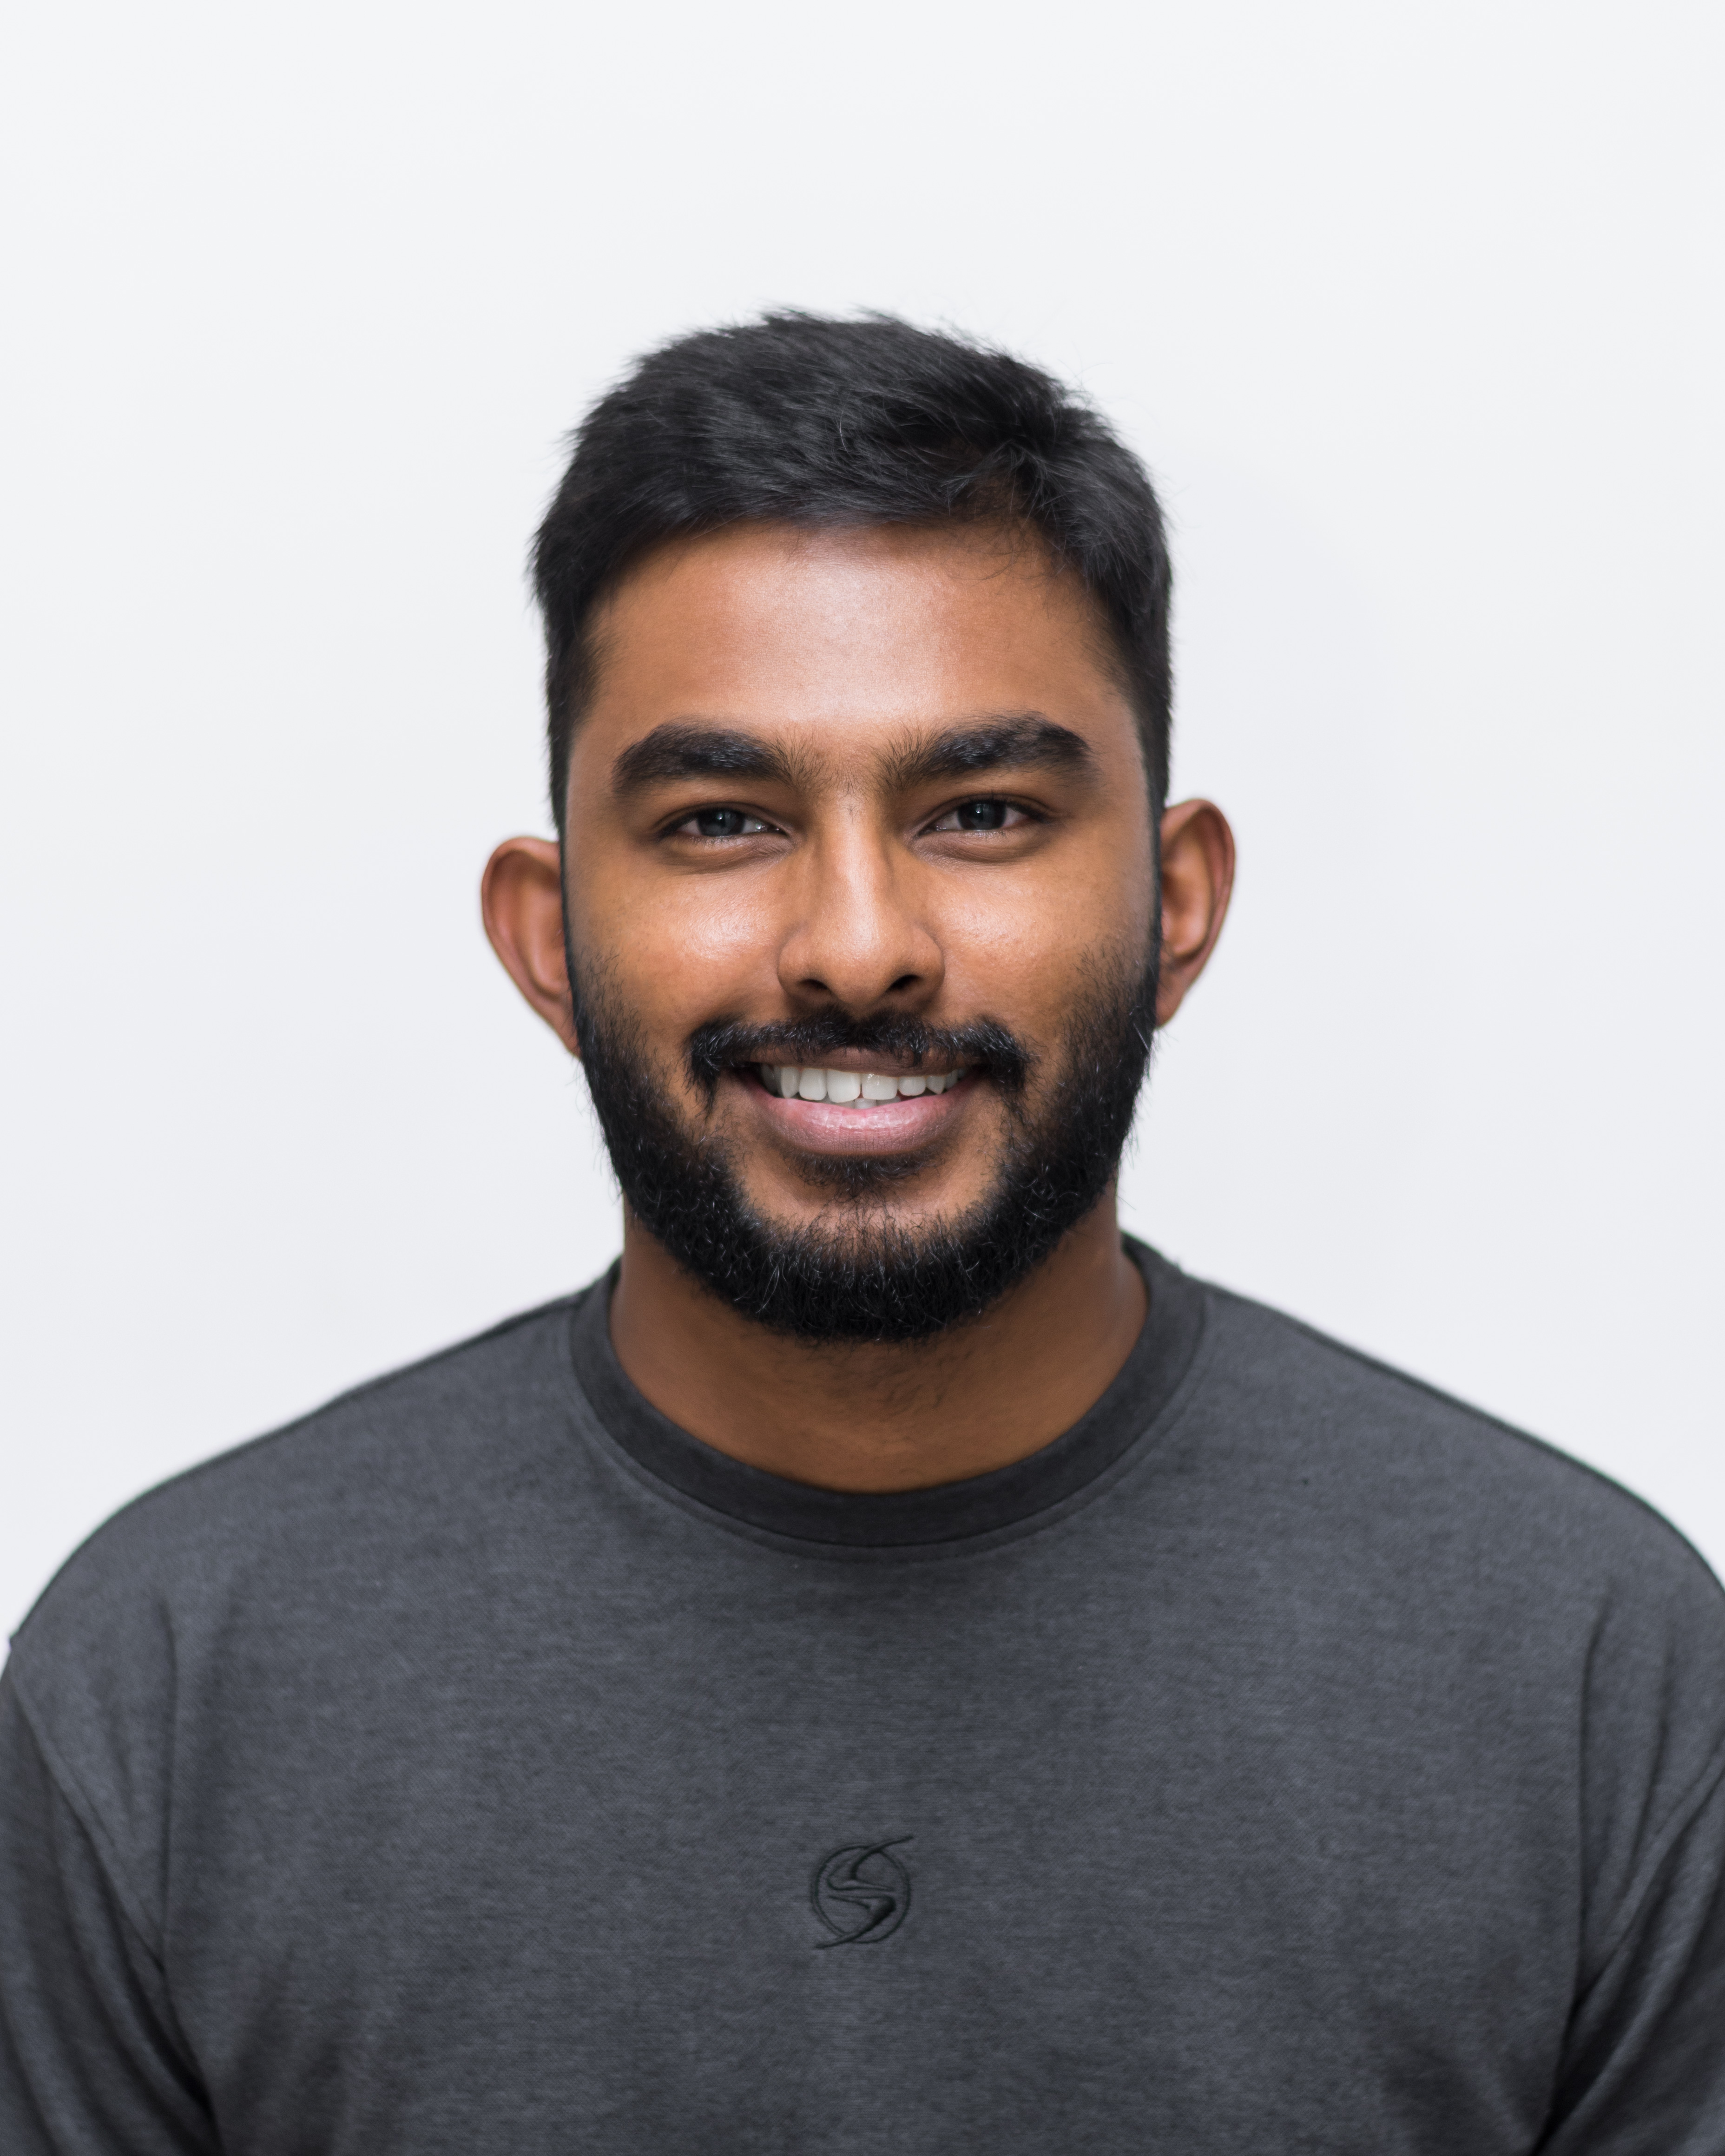
\includegraphics[width=2.7cm,height=3.3cm,keepaspectratio]{DSC_6741.JPG}}
\end{minipage}

\vspace{6pt}

% Personal details (no section heading — standard on many CVs)
\noindent
{\footnotesize \textbf{Birth:} 11/10/2001 \ \textbar\ \textbf{Place:} Kandy, Sri Lanka \ \textbar\ \textbf{Nationality:} Sri Lankan \ \textbar\ \textbf{Gender:} Male \ \textbar\ \textbf{Passport:} N6964000}
\end{tcolorbox}

\vspace{8pt}
\noindent
{\normalsize \textbf{Profile:} Full Stack Developer experienced in designing scalable applications with a strong focus on system architecture, abstraction, and efficient data flow. Applies a conceptual approach to building maintainable, high-performance systems, with practical experience in AI-driven automation and graph-based workflows.\par}

\vspace{2pt}

% ── EDUCATION ───────────────────────────────────────────────
\cvsection{Education}

\cvrow{2021\,--\,2024}{%
  \textbf{BSc (Hons) Information Technology Specializing in Software Engineering}
  {\newline\normalsize Sri Lanka Institute of Information Technology (SLIIT), Colombo}\\[1pt]
  \hfill{\normalsize\textit{GPA: 3.47\,/\,4.0 $\mid$ EQF Level\,6}}\\[1pt]
  {\small Core Modules: Software Architecture, Machine Learning, Cloud Computing,
  Distributed Systems, Mobile Development, Database Design}}

\cvrow{2018\,--\,2020}{%
  \textbf{G.C.E. Advanced Level (A/L)} - Physical Science Stream
  \newline{\normalsize Kingswood College, Kandy}}

\cvrow{2007\,--\,2017}{%
  \textbf{G.C.E. Ordinary Level (O/L)}
  {\newline\normalsize Kingswood College, Kandy}}

% ── RESEARCH & PUBLICATIONS ─────────────────────────────────
\cvsection{Research \& Publications}

\vspace{2pt}
\noindent{\color{MidGray}12/2024} \textbar\ \textbf{Conference Paper: International Conference on Advancements in Computing (ICAC)}\\[2pt]
{\small
\textbf{Title:} Adaptive Learning Tool to Enhance Educational Outcomes for Students with Inattentive Attention Deficit Hyperactivity Disorder (ADHD)\\
\textbf{Role:} Lead Researcher / Presenter\\
\textbf{Details:} Investigated AI-based educational interventions for cognitive support. Published by IEEE.\\
\textbf{Identifier:} DOI: 10.1109/ICAC64487.2024.10850982\par}

% ── ACADEMIC PROJECTS ───────────────────────────────────────
\cvsection{Academic Projects}

\vspace{2pt}
\noindent\textbf{BrainStation - Adaptive Quizzing Tool}\\[2pt]
{\small Adaptive learning tool for ADHD students. Developed quiz generation, dynamic UI, and modified algorithm to improve memory retention, handling full frontend \& backend.\\
\textit{Links:} {\footnotesize\href{https://bit.ly/3zigiPH}{GitHub (Backend)} \textbar\ \href{https://bit.ly/3Bqgf4E}{GitHub (Frontend)} \textbar\ \href{https://bit.ly/3ZFUxUm}{GitHub (Admin)} \textbar\ \href{https://bit.ly/4dgAZcB}{Figma}}\\[1pt]
\stack{AI/ML \textperiodcentered\ NLP/T5 \textperiodcentered\ Node.js \textperiodcentered\ React.js \textperiodcentered\ TailwindCSS \textperiodcentered\ MongoDB \textperiodcentered\ Firebase}\par}

\vspace{6pt}
\noindent\textbf{AutoCare Xpress - Car Servicing App}\\[2pt]
{\small Streamlined car service appointments with flexible scheduling and real-time updates. Designed UI and integrated Firebase for station registration, image uploads, and push notifications.\\
\textit{Links:} {\footnotesize\href{https://bit.ly/4gteunD}{GitHub} \textbar\ \href{https://bit.ly/3Zw2DPp}{Figma}}\\[1pt]
\stack{React Native \textperiodcentered\ Firebase (RealtimeDB \& FCM) \textperiodcentered\ Expo}\par}

\vspace{6pt}
\noindent\textbf{TraveloThreads - Travel Enthusiast Social App}\\[2pt]
{\small Travel-focused social platform with posts, images, and location tags. Added interactive features (likes, comments), Firestore Security Rules, and indexing for scalability.\\
\textit{Links:} {\footnotesize\href{https://bit.ly/3Bni0Q6}{GitHub} \textbar\ \href{https://bit.ly/3TFG1rZ}{Figma}}\\[1pt]
\stack{SwiftUI \textperiodcentered\ Rive \textperiodcentered\ Firebase \textperiodcentered\ Cocoapods}\par}

\newpage
% ── PROFESSIONAL EXPERIENCE ─────────────────────────────────
\cvsection{Professional Experience}

\cvrow{05/2025\,--\,Present}{%
  \textbf{Software Engineer} \textbar\ Pearson Lanka (Pvt) Ltd, Colombo\\[-2pt]
  \cvlist{
    \item Developed scalable frontend systems using React, TypeScript, and Vite for Pearson+ eText
    \item Designed component-driven architecture with reusable UI modules and custom hooks
    \item Engineered extensible widget system and built encapsulated components using Shadow DOM
    \item Applied security best practices to mitigate XSS; ensured cross-browser compatibility
  }
  \stack{React \textperiodcentered\ TypeScript \textperiodcentered\ Vite \textperiodcentered\ Redux}}

\cvrow{12/2024\,--\,05/2025}{%
  \textbf{Software Engineer} \textbar\ CodeGen International (Pvt) Ltd, Colombo\\[-2pt]
  \cvlist{
    \item Developed Java-based microservices for core backend systems and integrated enterprise services
    \item Engineered RAG-based system using LangChain and LangGraph with retrieval pipelines
    \item Designed internal automation platform; orchestrated CI/CD pipelines and automated deployments
  }
  \stack{Java \textperiodcentered\ Spring Boot \textperiodcentered\ Python \textperiodcentered\ LangChain \textperiodcentered\ LangGraph \textperiodcentered\ SOAP \textperiodcentered\ CI/CD}}

\cvrow{04/2023\,--\,04/2024}{%
  \textbf{Software Engineer Intern} \textbar\ Pearson Lanka (Pvt) Ltd, Colombo\\[-2pt]
  \cvlist{
    \item Developed UI features using React, Redux, SCSS, and Material-UI
    \item Migrated legacy code to React functional components and hooks; refactored into modular structures
    \item Improved state management using Redux Toolkit and modern patterns
  }
  \stack{React.js \textperiodcentered\ Redux Toolkit \textperiodcentered\ SCSS \textperiodcentered\ Material-UI}}

% ── COMMUNITY & VOLUNTEERING ────────────────────────────────
\cvsection{Community \& Volunteering}

\cvrow{2023\,--\,2024}{%
  \textbf{Director of Developer Relations} \textbar\ SLIIT Mozilla Club\\
  {\small Led community engagement; developed the club's official website;
  organized and delivered technical talks and knowledge-sharing events.}}

\cvrow{2022\,--\,2023}{%
  \textbf{Project Coordinator (Head Board)} \textbar\ SLIIT FOSS Community\\
  {\small Coordinated open-source development projects across a multi-team
  developer community; mentored junior contributors.}}

% ── LANGUAGE SKILLS ─────────────────────────────────────────
\cvsection{Language Skills}

\noindent
\begin{tabularx}{\linewidth}{@{}X X@{}}
  \textbf{Sinhala:} Native &
  \textbf{English:} C1 - Professional Working Proficiency \\
\end{tabularx}

% ── SKILLS ──────────────────────────────────────────────────
\cvsection{Skills \& Competencies}

\noindent
\begin{tabularx}{\linewidth}{@{} p{2.5cm} X @{}}
  \textbf{Backend}   & Java, Node.js, Express.js, Python, REST APIs, SOAP, Microservices\\[2pt]
  \textbf{Frontend}  & React.js, TypeScript, JavaScript, React Native, Redux,
                       Material-UI, TailwindCSS, SCSS\\[2pt]
  \textbf{AI\,/\,ML} & LangChain, LangGraph, RAG Pipelines, OpenAI API,
                       NLP, Vector Embeddings\\[2pt]
  \textbf{DevOps}    & Docker, Git, CI/CD (GitHub Actions), Firebase, MongoDB, SQL\\[2pt]
  \textbf{Other}     & Swift, SwiftUI, Rive, Figma, Agile/Scrum\\
\end{tabularx}

% ── NON-RELATIVE REFEREES ───────────────────────────────────
\cvsection{References}

\noindent
\begin{tabularx}{\linewidth}{@{}X X@{}}
  \textbf{Dr. Dinuka Wijendra}, PhD &
  \textbf{Prof. Anuradha Jayakody} \\
  Senior Lecturer (Higher Grade) &
  Professor \& Head of Department \\
  Faculty of Computing, SLIIT &
  Faculty of Computing, SLIIT \\
  \href{mailto:dinuka.w@sliit.lk}{dinuka.w@sliit.lk} &
  \href{mailto:anuradha.j@sliit.lk}{anuradha.j@sliit.lk} \\
  (+94) 71 952 5253 &
  (+94) 71 490 0228 \\
\end{tabularx}

% ── SIGNATURE BLOCK ─────────────────────────────────────────
\vfill

\vspace{10pt}
% Add scanned signature: \includegraphics[height=1.3cm]{signature.png}\\[-4pt]
\noindent\rule{5.0cm}{0.4pt}\\[2pt]
{\small Danuja Hemal Jayasuriya}

\end{document}
